For the scaling functions we find at this order:
\begin{align}
\bar c_{\tVA,xF_3,\Pg}^{(1)} &= \bar c_{\tVA,g_4,\Pg}^{(1)} = \bar c_{\tVA,g_L,\Pg}^{(1)} = 0
\end{align}
and 
\begin{align}
\bar c_{\tVV,2xg_1,\Pg}^{(1)} &= \bar c_{\tAA,2xg_1,\Pg}^{(1)}
\end{align}
and furthermore  near threshold, we find
\begin{equation}
\bar c_{\vec k,\Pg}^{(1),\tThr} = c_{\vec k,\Pg}^{(0),\text{thr}} \frac{1}{\pi^2}
     C_A\left(\bar a_{\vec k,\Pg}^{(1,1)}\ln(\beta) + \bar a_{\vec k,\Pg}^{(1,0)}\right)\;,
\end{equation} 
with
\begin{align}
\bar a^{(1,1)}_{\vec k,\Pg} &= -\frac 1 2\\
\bar a^{(1,0)}_{\tVV,F_2,\Pg} &= -\frac 1 4 \ln\left(\frac{16\chi_q}{(1+\chi_q)^2}\right)+\frac 1 2\\
\bar a^{(1,0)}_{\tVV,F_L,\Pg} &= \bar a^{(1,0)}_{\tVV,F_2,\Pg} + \frac 1 6\\
\bar a^{(1,0)}_{\tVV,2xg_1,\Pg} &= \bar a^{(1,0)}_{\tAA,F_2,\Pg} = \bar a^{(1,0)}_{\tAA,F_L,\Pg} = \bar a^{(1,0)}_{\tAA,2xg_1,\Pg}= \bar a^{(1,0)}_{\tVV,F_2,\Pg}
\end{align}

\begin{figure}[ht!]
\centering
\begin{subfigure}[t]{.3\textwidth}
	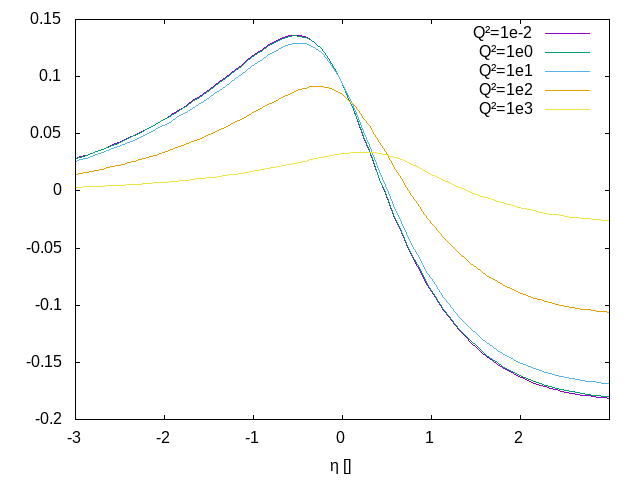
\includegraphics[width=\textwidth]{../../img2/partonic/cgBar1_VV_F2}
\end{subfigure}%
\begin{subfigure}[t]{.3\textwidth}
	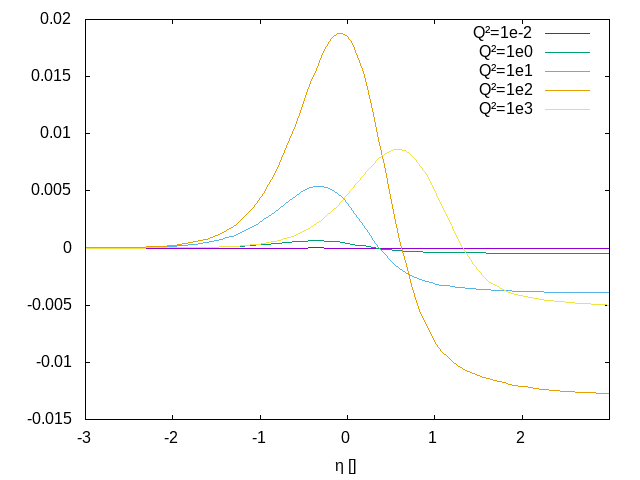
\includegraphics[width=\textwidth]{../../img2/partonic/cgBar1_VV_FL}
\end{subfigure}%
\begin{subfigure}[t]{.3\textwidth}
	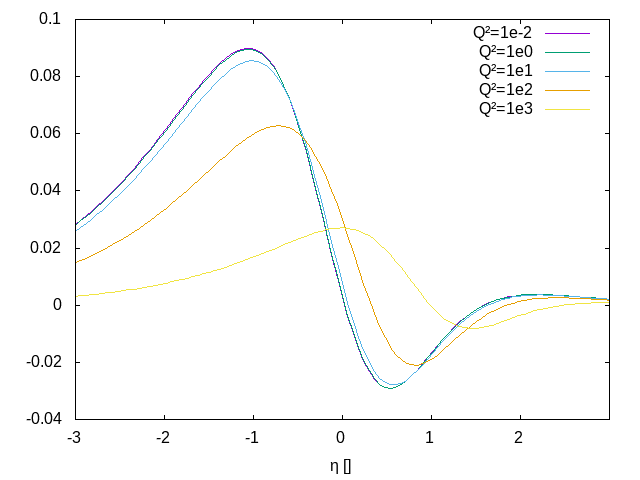
\includegraphics[width=\textwidth]{../../img2/partonic/cgBar1_VV_x2g1}
\end{subfigure}\\%
\begin{subfigure}[t]{.3\textwidth}
	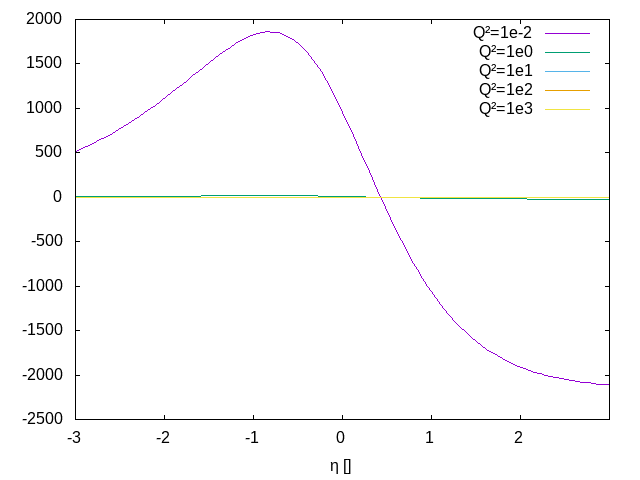
\includegraphics[width=\textwidth]{../../img2/partonic/cgBar1_AA_F2}
\end{subfigure}%
\begin{subfigure}[t]{.3\textwidth}
	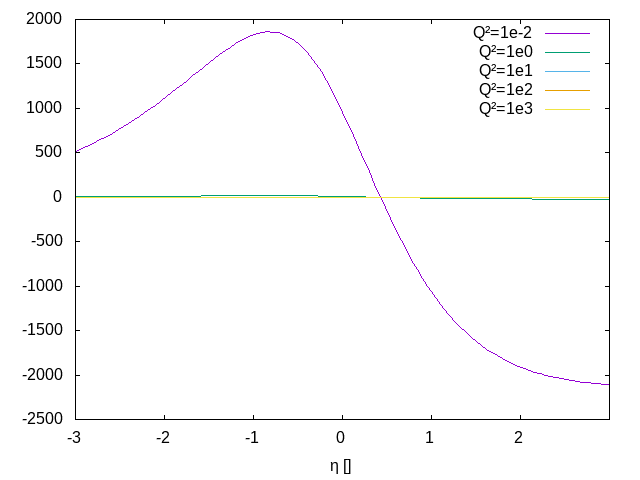
\includegraphics[width=\textwidth]{../../img2/partonic/cgBar1_AA_FL}
\end{subfigure}%
\begin{subfigure}[t]{.3\textwidth}
	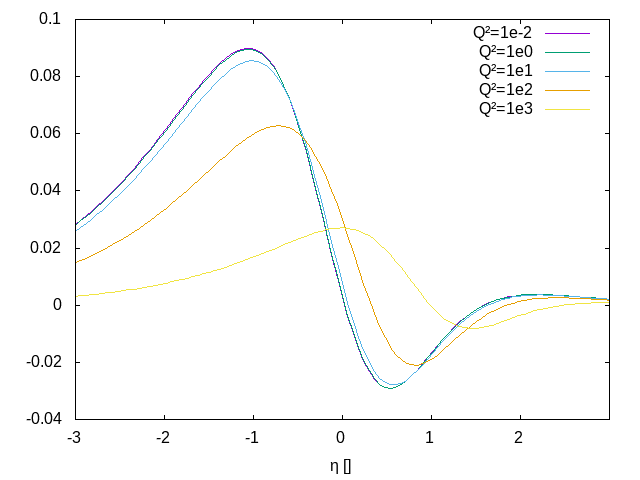
\includegraphics[width=\textwidth]{../../img2/partonic/cgBar1_AA_x2g1}
\end{subfigure}%
\caption{next-to-leading order scaling functions $\bar c_{k,\Pg}^{(1)}(\eta,\xi)$ plotted as function of $\eta=s/(4m^2)-1$ for different values of $Q^2$ in units of $\si{\GeV^2}$ at $m=\SI{4.75}{\GeV}$ (i.e. different values of $\xi=Q^2/m^2$) }\label{fig:cgBar1}
\end{figure}
